\section{Цель работы}
	Разработать экспертную систему с использованием среды CLIPS.
	
\section{Предметная область}
	Целевая ЭС выполняет функцию оценки платформ для социальной торговли. Социальная торговля -- онлайн-трейдинг на финансовых рынках в рамках социальной платформы, внутри которой трейдеры взаимодействуют друг с другом.
	
	На рисунке \ref{tree} изображено дерево целей экспертной системы. Дугами отмечены вершины И, отсутствием дуг ИЛИ.
	
	\begin{figure}[ht] 
		\center
		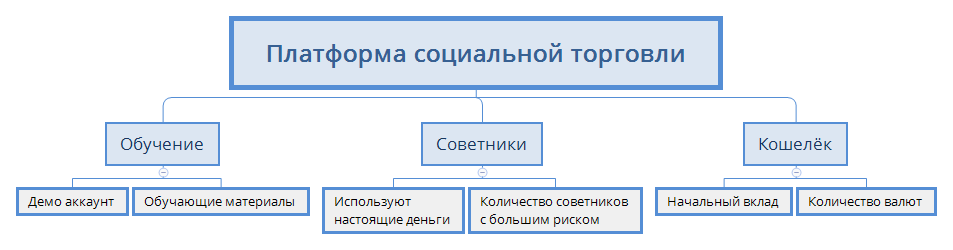
\includegraphics [width=\textwidth] {social-trading}
		\caption{Дерево целей} 
		\label{tree}
	\end{figure}
	\FloatBarrier

	На основе дерева целей описаны переменные и правила, представленные в листинге.
	
	Фактор уверенности для операции <<И>> вычисляется по формуле $(a * b) / 100$, а для правила <<ИЛИ>> - по формуле 	$a + b - (a * b) / 100$
	
\newpage	
\section{Листинг}

	\lstinputlisting[language=Lisp, caption={Листинг программы}]{listings/st.clp}

\newpage
\section{Примеры выполнения}

	Для начала работы необходимо загрузить программу в консоль CLIPS. Делается это с помощью команды \textit{load}, как показано в листинге \ref{loading}.
	
	\lstinputlisting[caption={Загрузка программы}, label=loading]{listings/load.txt}

	В листинге \ref{good} приведён пример платформы с высоким рейтингом, а в листинге \ref{bad} - с низким.

	\lstinputlisting[caption={Платформа с высоким рейтингом}, label=good]{listings/success.txt}

	\lstinputlisting[caption={Платформа с низким рейтингом}, label=bad]{listings/failure.txt}

\section{Вывод}
	В результате данной работы была спроектирована разработана ЭС, которая позволяет дать экспертную оценку платформам социальной торговли по введенным параметрам. Изучена программа для создания экспертных систем CLIPS.